\documentclass[]{article}
\usepackage{lmodern}
\usepackage{amssymb,amsmath}
\usepackage{ifxetex,ifluatex}
\usepackage{fixltx2e} % provides \textsubscript
\ifnum 0\ifxetex 1\fi\ifluatex 1\fi=0 % if pdftex
  \usepackage[T1]{fontenc}
  \usepackage[utf8]{inputenc}
\else % if luatex or xelatex
  \ifxetex
    \usepackage{mathspec}
  \else
    \usepackage{fontspec}
  \fi
  \defaultfontfeatures{Ligatures=TeX,Scale=MatchLowercase}
\fi
% use upquote if available, for straight quotes in verbatim environments
\IfFileExists{upquote.sty}{\usepackage{upquote}}{}
% use microtype if available
\IfFileExists{microtype.sty}{%
\usepackage{microtype}
\UseMicrotypeSet[protrusion]{basicmath} % disable protrusion for tt fonts
}{}
\usepackage[margin=1in]{geometry}
\usepackage{hyperref}
\hypersetup{unicode=true,
            pdftitle={Biostats\_Methods\_hw1},
            pdfauthor={Yishan Wang},
            pdfborder={0 0 0},
            breaklinks=true}
\urlstyle{same}  % don't use monospace font for urls
\usepackage{color}
\usepackage{fancyvrb}
\newcommand{\VerbBar}{|}
\newcommand{\VERB}{\Verb[commandchars=\\\{\}]}
\DefineVerbatimEnvironment{Highlighting}{Verbatim}{commandchars=\\\{\}}
% Add ',fontsize=\small' for more characters per line
\usepackage{framed}
\definecolor{shadecolor}{RGB}{248,248,248}
\newenvironment{Shaded}{\begin{snugshade}}{\end{snugshade}}
\newcommand{\KeywordTok}[1]{\textcolor[rgb]{0.13,0.29,0.53}{\textbf{#1}}}
\newcommand{\DataTypeTok}[1]{\textcolor[rgb]{0.13,0.29,0.53}{#1}}
\newcommand{\DecValTok}[1]{\textcolor[rgb]{0.00,0.00,0.81}{#1}}
\newcommand{\BaseNTok}[1]{\textcolor[rgb]{0.00,0.00,0.81}{#1}}
\newcommand{\FloatTok}[1]{\textcolor[rgb]{0.00,0.00,0.81}{#1}}
\newcommand{\ConstantTok}[1]{\textcolor[rgb]{0.00,0.00,0.00}{#1}}
\newcommand{\CharTok}[1]{\textcolor[rgb]{0.31,0.60,0.02}{#1}}
\newcommand{\SpecialCharTok}[1]{\textcolor[rgb]{0.00,0.00,0.00}{#1}}
\newcommand{\StringTok}[1]{\textcolor[rgb]{0.31,0.60,0.02}{#1}}
\newcommand{\VerbatimStringTok}[1]{\textcolor[rgb]{0.31,0.60,0.02}{#1}}
\newcommand{\SpecialStringTok}[1]{\textcolor[rgb]{0.31,0.60,0.02}{#1}}
\newcommand{\ImportTok}[1]{#1}
\newcommand{\CommentTok}[1]{\textcolor[rgb]{0.56,0.35,0.01}{\textit{#1}}}
\newcommand{\DocumentationTok}[1]{\textcolor[rgb]{0.56,0.35,0.01}{\textbf{\textit{#1}}}}
\newcommand{\AnnotationTok}[1]{\textcolor[rgb]{0.56,0.35,0.01}{\textbf{\textit{#1}}}}
\newcommand{\CommentVarTok}[1]{\textcolor[rgb]{0.56,0.35,0.01}{\textbf{\textit{#1}}}}
\newcommand{\OtherTok}[1]{\textcolor[rgb]{0.56,0.35,0.01}{#1}}
\newcommand{\FunctionTok}[1]{\textcolor[rgb]{0.00,0.00,0.00}{#1}}
\newcommand{\VariableTok}[1]{\textcolor[rgb]{0.00,0.00,0.00}{#1}}
\newcommand{\ControlFlowTok}[1]{\textcolor[rgb]{0.13,0.29,0.53}{\textbf{#1}}}
\newcommand{\OperatorTok}[1]{\textcolor[rgb]{0.81,0.36,0.00}{\textbf{#1}}}
\newcommand{\BuiltInTok}[1]{#1}
\newcommand{\ExtensionTok}[1]{#1}
\newcommand{\PreprocessorTok}[1]{\textcolor[rgb]{0.56,0.35,0.01}{\textit{#1}}}
\newcommand{\AttributeTok}[1]{\textcolor[rgb]{0.77,0.63,0.00}{#1}}
\newcommand{\RegionMarkerTok}[1]{#1}
\newcommand{\InformationTok}[1]{\textcolor[rgb]{0.56,0.35,0.01}{\textbf{\textit{#1}}}}
\newcommand{\WarningTok}[1]{\textcolor[rgb]{0.56,0.35,0.01}{\textbf{\textit{#1}}}}
\newcommand{\AlertTok}[1]{\textcolor[rgb]{0.94,0.16,0.16}{#1}}
\newcommand{\ErrorTok}[1]{\textcolor[rgb]{0.64,0.00,0.00}{\textbf{#1}}}
\newcommand{\NormalTok}[1]{#1}
\usepackage{graphicx,grffile}
\makeatletter
\def\maxwidth{\ifdim\Gin@nat@width>\linewidth\linewidth\else\Gin@nat@width\fi}
\def\maxheight{\ifdim\Gin@nat@height>\textheight\textheight\else\Gin@nat@height\fi}
\makeatother
% Scale images if necessary, so that they will not overflow the page
% margins by default, and it is still possible to overwrite the defaults
% using explicit options in \includegraphics[width, height, ...]{}
\setkeys{Gin}{width=\maxwidth,height=\maxheight,keepaspectratio}
\IfFileExists{parskip.sty}{%
\usepackage{parskip}
}{% else
\setlength{\parindent}{0pt}
\setlength{\parskip}{6pt plus 2pt minus 1pt}
}
\setlength{\emergencystretch}{3em}  % prevent overfull lines
\providecommand{\tightlist}{%
  \setlength{\itemsep}{0pt}\setlength{\parskip}{0pt}}
\setcounter{secnumdepth}{0}
% Redefines (sub)paragraphs to behave more like sections
\ifx\paragraph\undefined\else
\let\oldparagraph\paragraph
\renewcommand{\paragraph}[1]{\oldparagraph{#1}\mbox{}}
\fi
\ifx\subparagraph\undefined\else
\let\oldsubparagraph\subparagraph
\renewcommand{\subparagraph}[1]{\oldsubparagraph{#1}\mbox{}}
\fi

%%% Use protect on footnotes to avoid problems with footnotes in titles
\let\rmarkdownfootnote\footnote%
\def\footnote{\protect\rmarkdownfootnote}

%%% Change title format to be more compact
\usepackage{titling}

% Create subtitle command for use in maketitle
\newcommand{\subtitle}[1]{
  \posttitle{
    \begin{center}\large#1\end{center}
    }
}

\setlength{\droptitle}{-2em}

  \title{Biostats\_Methods\_hw1}
    \pretitle{\vspace{\droptitle}\centering\huge}
  \posttitle{\par}
    \author{Yishan Wang}
    \preauthor{\centering\large\emph}
  \postauthor{\par}
      \predate{\centering\large\emph}
  \postdate{\par}
    \date{2018-9-24}


\begin{document}
\maketitle

\section{Problem 1}\label{problem-1}

The name of the story I found online is called \textbf{``Lung Cancer
Screening Most Beneficial for Those at Highest Risk, Analysis
Suggests''}. The similar stories were reported in several media outlet,
but they were represented differently. In the story that I found, the
author uses the result of the experiment that was conducted to prove the
high-risk groups are more likely to be screened to diagnose one case of
lung cancer. The experimental screeing was done by a risk-based
approach. The experiement shows that aprroximatly 30 lung cancer
diagnoses were made from every 1,000 patients in the high-risk groups,
comparing with 5 diagnoses in the lowest-risk group. In another similar
story, the facts are listed as who should be screened. The people who
should be screened are the people who had a history of heavy smoking,
the people smoke now or have quit within the past 15 years and the
people between 55 and 80 years old. Based on this story, older people
are also more likely to have lung cancer to be diagnosed. By reading the
original reference, the experiment is the observational study because
the reseachers observe and predict the number of deaths due to lung
cancer. The sample selection is based on people's risk level. Risk level
is how likely one person will be diagnoses lung cancer. Two groups of
people are sampled. One is the group that has high risk level, and
another one is the group that has low risk level. The sample size is
selected properly. I think the only possible bias might be that
reseachers didn't consider other factors can affect people's risk level,
such as air pollution. The result is that people who are at high risk is
more likely to be screened lung cancer. I think I seriously should take
the results of the research after considering the possible bias that
mentioned above.

\textbf{References}

NCI. ``Lung Cancer Screening May Benefit Those at Highest Risk.''
National Cancer Institute, 28 Feb. 2018,
www.cancer.gov/news-events/cancer-currents-blog/2018/lung-cancer-screening-identifying-who-benefits.

Bach, Peter B., et al. ``Benchmarking Lung Cancer Mortality Rates in
Current and Former Smokers.'' Chest, vol.~126, no. 6, 2004,
pp.~1742-1749.

\section{Problem 2}\label{problem-2}

a). P(an adult having BDP \textgreater{}= 90mmHg at screening will
actually be hypertensive) = 75 / 100 = 0.75

b). P(an adult having DBP \textless{} 90mmHg at screening will not
actually be hypertensive) = 85 / 100 = 0.85

c). P(an adult in this community is truly hypertensive) = ((75 / 100) *
650 + (15 / 100) * 5350) / 6000 = 0.215

d). P(a hypertensive person will be found to have a DBP ??? 90mmHg at
the initial screening) = ((75 / 100) * 650) / ((75 / 100) * 650 + (15 /
100) * 5350) = 0.378

e). P(a non-hypertensive person will be found to have a DBP \textless{}
90mmHg at the initial screening) = ((85 / 100) * 5350) / ((25 / 650) *
650 + (85 / 100) * 5350) = 0.995

\section{Problem 3}\label{problem-3}

a). P(exactly half of selected men cannot distinguish between red and
green) = dbinom(5, 10, 0.08) = 5.4423894\times 10\^{}\{-4\}

b). P(exactly half of selected women cannot distinguish between red and
green) = dbinom(5, 10, 0.3) = 0.1029193

The probability increased. The probability of selecting exactly half of
selected women who cannot distinguish between red and green is bigger
than the probability of selecting exactly half of selected men who
cannot distinguish between red and green.

Note: Binomial formula is attached at the end of the document.

\section{Problem 4}\label{problem-4}

a). Let X be the number of cases occur in a given year in New York City

P(X = 30) = dpois(30, 8.55 * 5) = 0.0086763

b). Let Y1 be the number of non-Hispanic whites cases occur in a given
year in New York City

Let Y2 be the number of Black cases occur in a given year in New York
City

Let Y3 be the number of Asian cases occur in a given year in New York
City

P(Y1 = 30) = dpois(30, 8.55 * 0.446 * 6.02) = 0.0271376

P(Y2 = 30) = dpois(30, 8.55 * 0.251 * 0.31) =
9.4942431\times 10\^{}\{-39\}

P(Y3 = 30) = dpois(30, 8.55 * 0.118 * 0.39) =
1.7899443\times 10\^{}\{-45\}

The probability of 30 cases of uniform racial group (non-Hispanic, Black
or Asian) occur in a given year in New York City is less than the
probability of 30 cases of mixed racial group occur in a given year in
New York City.

Note: Poisson formula is attached at the end of the document.

\section{Problem 5}\label{problem-5}

a). Since the variance is 25, the standard deviation is 5. The value
that is 1 standard deviation above the mean is 35 + 5 = 40. The value
that is 1 standard deviation below the mean is 35 - 5 = 30. The values
that are 2 standard deviation away from the mean are 35 +- 5*2, which
are 25 and 45.

b). Let X be the time for a dental cleaning procedure

Since the distribution of duration time for this procedure is
approximately normal, we standardize X to Z.

P(25 \textless{} X \textless{} 45) = P((25 - 35) / 5 \textless{} (X -
mu) / sigma \textless{} (45 - 35) / 5) = P(-2 \textless{} Z \textless{}
2) = 0.9544997

c). P(X \textless{} 20) + P(X \textgreater{} 50) = P((X - mu) / sigma
\textless{} (20 - 35) / 5) + P((X - mu) / sigma \textgreater{} (50 - 35)
/ 5) = P(Z \textless{} -3) + P(Z \textgreater{} 3) = 0.0026998

d). E(Z) = E((X - mu) / sigma) = (1 / sigma) * E(X - mu) = (1 / sigma) *
(E(X) - mu) = (1 / 5) * (35 - 35) = 0

Var(Z) = Var((X - mu) / sigma) = (1 / sigma\^{}2) * Var(Z - mu) = (1 /
sigma\^{}2) * Var(Z) = (1 / 25) * 25 = 1

\section{Problem 6}\label{problem-6}

a).

Import data frame to R

\begin{Shaded}
\begin{Highlighting}[]
\NormalTok{migraine_data =}\StringTok{ }\KeywordTok{read_excel}\NormalTok{(}\StringTok{"./Migraine.xlsx"}\NormalTok{)}
\end{Highlighting}
\end{Shaded}

Arrange data frame by varibale Migraine

\begin{Shaded}
\begin{Highlighting}[]
\KeywordTok{arrange}\NormalTok{(migraine_data, migraine_data}\OperatorTok{$}\NormalTok{Migraine)}
\end{Highlighting}
\end{Shaded}

\begin{verbatim}
## # A tibble: 419 x 5
##    Migraine  CESD NDDIE `ABNAS memory` `ABNAS language`
##       <dbl> <dbl> <dbl>          <dbl>            <dbl>
##  1        0    42    NA              1                0
##  2        0    NA     6              0                0
##  3        0    10    11              0                0
##  4        0    NA    NA              1                0
##  5        0    23    16              1                0
##  6        0     6     8              1                0
##  7        0    NA    NA              0                0
##  8        0    NA    NA              2                0
##  9        0    NA    NA              0                0
## 10        0    NA    NA              4                0
## # ... with 409 more rows
\end{verbatim}

Subset from arranged data frame to a data frame with migraine and a data
frame without migraine

\begin{Shaded}
\begin{Highlighting}[]
\NormalTok{sub_}\DecValTok{1}\NormalTok{ =}\StringTok{ }\KeywordTok{subset}\NormalTok{(migraine_data, migraine_data}\OperatorTok{$}\NormalTok{Migraine }\OperatorTok{==}\StringTok{ }\DecValTok{1}\NormalTok{)}
\NormalTok{sub_}\DecValTok{0}\NormalTok{ =}\StringTok{ }\KeywordTok{subset}\NormalTok{(migraine_data, migraine_data}\OperatorTok{$}\NormalTok{Migraine }\OperatorTok{==}\StringTok{ }\DecValTok{0}\NormalTok{)}
\end{Highlighting}
\end{Shaded}

\subsection{Epilepsy patients with
migraine}\label{epilepsy-patients-with-migraine}

Count NA of each variable of epilepsy patients with migraine

\begin{Shaded}
\begin{Highlighting}[]
\NormalTok{na_count =}\StringTok{ }\KeywordTok{sapply}\NormalTok{(sub_}\DecValTok{1}\NormalTok{, }\ControlFlowTok{function}\NormalTok{(y) }\KeywordTok{sum}\NormalTok{(}\KeywordTok{length}\NormalTok{(}\KeywordTok{which}\NormalTok{(}\KeywordTok{is.na}\NormalTok{(y)))))}
\NormalTok{na_count =}\StringTok{ }\KeywordTok{data.frame}\NormalTok{(na_count)}
\NormalTok{na_count}
\end{Highlighting}
\end{Shaded}

\begin{verbatim}
##                na_count
## Migraine              0
## CESD                  8
## NDDIE                 9
## ABNAS memory          0
## ABNAS language        0
\end{verbatim}

Count sample size of the subset data frame before deleting NA

\begin{Shaded}
\begin{Highlighting}[]
\NormalTok{nrow_}\DecValTok{1}\NormalTok{ =}\StringTok{ }\KeywordTok{NROW}\NormalTok{(sub_}\DecValTok{1}\NormalTok{)}
\NormalTok{nrow_}\DecValTok{1}
\end{Highlighting}
\end{Shaded}

\begin{verbatim}
## [1] 82
\end{verbatim}

Delete NA from data frame with migranie

\begin{Shaded}
\begin{Highlighting}[]
\NormalTok{sub_1_omit =}\StringTok{ }\KeywordTok{na.omit}\NormalTok{(sub_}\DecValTok{1}\NormalTok{)}
\end{Highlighting}
\end{Shaded}

Count new sample size after deleting NA

\begin{Shaded}
\begin{Highlighting}[]
\NormalTok{nrow_1_omit =}\StringTok{ }\KeywordTok{NROW}\NormalTok{(sub_1_omit)}
\NormalTok{nrow_1_omit}
\end{Highlighting}
\end{Shaded}

\begin{verbatim}
## [1] 73
\end{verbatim}

Find the number of rows are deleted

\begin{Shaded}
\begin{Highlighting}[]
\NormalTok{n_drop_}\DecValTok{1}\NormalTok{ =}\StringTok{ }\NormalTok{nrow_}\DecValTok{1} \OperatorTok{-}\StringTok{ }\NormalTok{nrow_1_omit}
\NormalTok{n_drop_}\DecValTok{1}
\end{Highlighting}
\end{Shaded}

\begin{verbatim}
## [1] 9
\end{verbatim}

Summerize the variables for epilepsy patients with migraine

\begin{Shaded}
\begin{Highlighting}[]
\NormalTok{dis_data_}\DecValTok{1}\NormalTok{ =}\StringTok{ }\KeywordTok{list}\NormalTok{(sub_1_omit}\OperatorTok{$}\NormalTok{CESD, sub_1_omit}\OperatorTok{$}\NormalTok{NDDIE, sub_1_omit}\OperatorTok{$}\StringTok{`}\DataTypeTok{ABNAS memory}\StringTok{`}\NormalTok{, sub_1_omit}\OperatorTok{$}\StringTok{`}\DataTypeTok{ABNAS language}\StringTok{`}\NormalTok{)}

\NormalTok{min =}\StringTok{ }\KeywordTok{sapply}\NormalTok{(dis_data_}\DecValTok{1}\NormalTok{, min)}
\NormalTok{max =}\StringTok{ }\KeywordTok{sapply}\NormalTok{(dis_data_}\DecValTok{1}\NormalTok{, max)}
\NormalTok{mean =}\StringTok{ }\KeywordTok{sapply}\NormalTok{(dis_data_}\DecValTok{1}\NormalTok{, mean)}
\NormalTok{median =}\StringTok{ }\KeywordTok{sapply}\NormalTok{(dis_data_}\DecValTok{1}\NormalTok{, median)}
\NormalTok{sd =}\StringTok{ }\KeywordTok{sapply}\NormalTok{(dis_data_}\DecValTok{1}\NormalTok{, sd)}
\NormalTok{IQR =}\StringTok{ }\KeywordTok{sapply}\NormalTok{(dis_data_}\DecValTok{1}\NormalTok{, IQR)}

\NormalTok{description =}\StringTok{ }\KeywordTok{rbind}\NormalTok{(min, max, mean, median, sd, IQR)}
\KeywordTok{colnames}\NormalTok{(description) =}\StringTok{ }\KeywordTok{c}\NormalTok{(}\StringTok{"CESD"}\NormalTok{, }\StringTok{"NDDIE"}\NormalTok{, }\StringTok{"ABNAS_memory"}\NormalTok{, }\StringTok{"ABNAS_language"}\NormalTok{)}
\NormalTok{description}
\end{Highlighting}
\end{Shaded}

\begin{verbatim}
##            CESD     NDDIE ABNAS_memory ABNAS_language
## min     0.00000  6.000000     0.000000       0.000000
## max    46.00000 23.000000    12.000000       8.000000
## mean   14.31507 11.424658     3.287671       1.890411
## median 11.00000 11.000000     2.000000       1.000000
## sd     11.52880  4.361822     3.449958       2.092059
## IQR    14.00000  6.000000     4.000000       3.000000
\end{verbatim}

\begin{Shaded}
\begin{Highlighting}[]
\NormalTok{prop_NDDIE_}\DecValTok{1}\NormalTok{ =}\StringTok{ }\KeywordTok{count}\NormalTok{(sub_1_omit, NDDIE }\OperatorTok{>=}\StringTok{ }\DecValTok{16}\NormalTok{) }\OperatorTok{/}\StringTok{ }\NormalTok{nrow_1_omit}
\NormalTok{prop_CESD_}\DecValTok{1}\NormalTok{ =}\StringTok{ }\KeywordTok{count}\NormalTok{(sub_1_omit, CESD }\OperatorTok{>=}\StringTok{ }\DecValTok{16}\NormalTok{) }\OperatorTok{/}\StringTok{ }\NormalTok{nrow_1_omit}

\NormalTok{prop_NDDIE_}\DecValTok{1}
\end{Highlighting}
\end{Shaded}

\begin{verbatim}
##   NDDIE >= 16         n
## 1  0.00000000 0.8493151
## 2  0.01369863 0.1506849
\end{verbatim}

\begin{Shaded}
\begin{Highlighting}[]
\NormalTok{prop_CESD_}\DecValTok{1}
\end{Highlighting}
\end{Shaded}

\begin{verbatim}
##   CESD >= 16         n
## 1 0.00000000 0.6575342
## 2 0.01369863 0.3424658
\end{verbatim}

P(NDDIE \textgreater{}= 16) = 0.1506849

P(CESD \textgreater{}= 16) = 0.3424658

\subsection{Epilepsy patients without
migraine}\label{epilepsy-patients-without-migraine}

Count NA of each variable of epilepsy patients without migraine

\begin{Shaded}
\begin{Highlighting}[]
\NormalTok{na_count =}\StringTok{ }\KeywordTok{sapply}\NormalTok{(sub_}\DecValTok{0}\NormalTok{, }\ControlFlowTok{function}\NormalTok{(y) }\KeywordTok{sum}\NormalTok{(}\KeywordTok{length}\NormalTok{(}\KeywordTok{which}\NormalTok{(}\KeywordTok{is.na}\NormalTok{(y)))))}
\NormalTok{na_count =}\StringTok{ }\KeywordTok{data.frame}\NormalTok{(na_count)}
\NormalTok{na_count}
\end{Highlighting}
\end{Shaded}

\begin{verbatim}
##                na_count
## Migraine              0
## CESD                 63
## NDDIE                64
## ABNAS memory          0
## ABNAS language        0
\end{verbatim}

Count sample size of the subset data frame before deleting NA

\begin{Shaded}
\begin{Highlighting}[]
\NormalTok{nrow_}\DecValTok{0}\NormalTok{ =}\StringTok{ }\KeywordTok{NROW}\NormalTok{(sub_}\DecValTok{0}\NormalTok{)}
\NormalTok{nrow_}\DecValTok{0}
\end{Highlighting}
\end{Shaded}

\begin{verbatim}
## [1] 337
\end{verbatim}

Delete NA from data frame without migranie

\begin{Shaded}
\begin{Highlighting}[]
\NormalTok{sub_0_omit =}\StringTok{ }\KeywordTok{na.omit}\NormalTok{(sub_}\DecValTok{0}\NormalTok{)}
\end{Highlighting}
\end{Shaded}

Count new sample size after deleting NA

\begin{Shaded}
\begin{Highlighting}[]
\NormalTok{nrow_0_omit =}\StringTok{ }\KeywordTok{NROW}\NormalTok{(sub_0_omit)}
\NormalTok{nrow_0_omit}
\end{Highlighting}
\end{Shaded}

\begin{verbatim}
## [1] 272
\end{verbatim}

Find the number of rows are deleted

\begin{Shaded}
\begin{Highlighting}[]
\NormalTok{n_drop_}\DecValTok{0}\NormalTok{ =}\StringTok{ }\NormalTok{nrow_}\DecValTok{0} \OperatorTok{-}\StringTok{ }\NormalTok{nrow_0_omit}
\NormalTok{n_drop_}\DecValTok{0}
\end{Highlighting}
\end{Shaded}

\begin{verbatim}
## [1] 65
\end{verbatim}

Summerize the variables for epilepsy patients without migraine

\begin{Shaded}
\begin{Highlighting}[]
\NormalTok{dis_data_}\DecValTok{0}\NormalTok{ =}\StringTok{ }\KeywordTok{list}\NormalTok{(sub_0_omit}\OperatorTok{$}\NormalTok{CESD, sub_0_omit}\OperatorTok{$}\NormalTok{NDDIE, sub_0_omit}\OperatorTok{$}\StringTok{`}\DataTypeTok{ABNAS memory}\StringTok{`}\NormalTok{, sub_0_omit}\OperatorTok{$}\StringTok{`}\DataTypeTok{ABNAS language}\StringTok{`}\NormalTok{)}

\NormalTok{min =}\StringTok{ }\KeywordTok{sapply}\NormalTok{(dis_data_}\DecValTok{0}\NormalTok{, min)}
\NormalTok{max =}\StringTok{ }\KeywordTok{sapply}\NormalTok{(dis_data_}\DecValTok{0}\NormalTok{, max)}
\NormalTok{mean =}\StringTok{ }\KeywordTok{sapply}\NormalTok{(dis_data_}\DecValTok{0}\NormalTok{, mean)}
\NormalTok{median =}\StringTok{ }\KeywordTok{sapply}\NormalTok{(dis_data_}\DecValTok{0}\NormalTok{, median)}
\NormalTok{sd =}\StringTok{ }\KeywordTok{sapply}\NormalTok{(dis_data_}\DecValTok{0}\NormalTok{, sd)}
\NormalTok{IQR =}\StringTok{ }\KeywordTok{sapply}\NormalTok{(dis_data_}\DecValTok{0}\NormalTok{, IQR)}

\NormalTok{description =}\StringTok{ }\KeywordTok{rbind}\NormalTok{(min, max, mean, median, sd, IQR)}
\KeywordTok{colnames}\NormalTok{(description) =}\StringTok{ }\KeywordTok{c}\NormalTok{(}\StringTok{"CESD"}\NormalTok{, }\StringTok{"NDDIE"}\NormalTok{, }\StringTok{"ABNAS_memory"}\NormalTok{, }\StringTok{"ABNAS_language"}\NormalTok{)}
\NormalTok{description}
\end{Highlighting}
\end{Shaded}

\begin{verbatim}
##            CESD     NDDIE ABNAS_memory ABNAS_language
## min     0.00000  6.000000     0.000000       0.000000
## max    48.00000 24.000000    12.000000       9.000000
## mean   10.52574 10.301471     2.639706       1.687500
## median  8.00000  9.000000     2.000000       1.000000
## sd     10.13886  4.489956     3.167344       2.282969
## IQR    11.00000  7.000000     4.000000       2.250000
\end{verbatim}

\begin{Shaded}
\begin{Highlighting}[]
\NormalTok{prop_NDDIE_}\DecValTok{0}\NormalTok{ =}\StringTok{ }\KeywordTok{count}\NormalTok{(sub_0_omit, NDDIE }\OperatorTok{>=}\StringTok{ }\DecValTok{16}\NormalTok{) }\OperatorTok{/}\StringTok{ }\NormalTok{nrow_0_omit}
\NormalTok{prop_CESD_}\DecValTok{0}\NormalTok{ =}\StringTok{ }\KeywordTok{count}\NormalTok{(sub_0_omit, CESD }\OperatorTok{>=}\StringTok{ }\DecValTok{16}\NormalTok{) }\OperatorTok{/}\StringTok{ }\NormalTok{nrow_0_omit}

\NormalTok{prop_NDDIE_}\DecValTok{0}
\end{Highlighting}
\end{Shaded}

\begin{verbatim}
##   NDDIE >= 16         n
## 1 0.000000000 0.8566176
## 2 0.003676471 0.1433824
\end{verbatim}

\begin{Shaded}
\begin{Highlighting}[]
\NormalTok{prop_CESD_}\DecValTok{0}
\end{Highlighting}
\end{Shaded}

\begin{verbatim}
##    CESD >= 16         n
## 1 0.000000000 0.7794118
## 2 0.003676471 0.2205882
\end{verbatim}

P(NDDIE \textgreater{}= 16) = 0.1433824

P(CESD \textgreater{}= 16) = 0.2205882

b).

\begin{Shaded}
\begin{Highlighting}[]
\KeywordTok{boxplot}\NormalTok{(}\KeywordTok{select}\NormalTok{(sub_1_omit, }\StringTok{"CESD"}\NormalTok{, }\StringTok{"NDDIE"}\NormalTok{, }\StringTok{"ABNAS memory"}\NormalTok{, }\StringTok{"ABNAS language"}\NormalTok{), }\DataTypeTok{ylab =} \StringTok{"Scores"}\NormalTok{, }\DataTypeTok{xlab =} \StringTok{"Epilepsy Patients Information"}\NormalTok{, }\DataTypeTok{main =} \StringTok{"Variables for Epilepsy Patients with Migraine"}\NormalTok{)}
\end{Highlighting}
\end{Shaded}

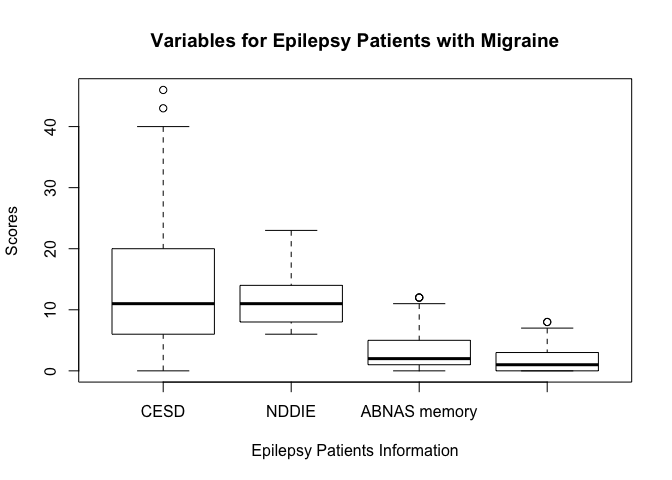
\includegraphics{Methods_hw1_files/figure-latex/unnamed-chunk-17-1.pdf}

\begin{Shaded}
\begin{Highlighting}[]
\KeywordTok{boxplot}\NormalTok{(}\KeywordTok{select}\NormalTok{(sub_0_omit, }\StringTok{"CESD"}\NormalTok{, }\StringTok{"NDDIE"}\NormalTok{, }\StringTok{"ABNAS memory"}\NormalTok{, }\StringTok{"ABNAS language"}\NormalTok{), }\DataTypeTok{ylab =} \StringTok{"Scores"}\NormalTok{, }\DataTypeTok{xlab =} \StringTok{"Epilepsy Patients Information"}\NormalTok{, }\DataTypeTok{main =} \StringTok{"Variables for Epilepsy Patients without Migraine"}\NormalTok{)}
\end{Highlighting}
\end{Shaded}

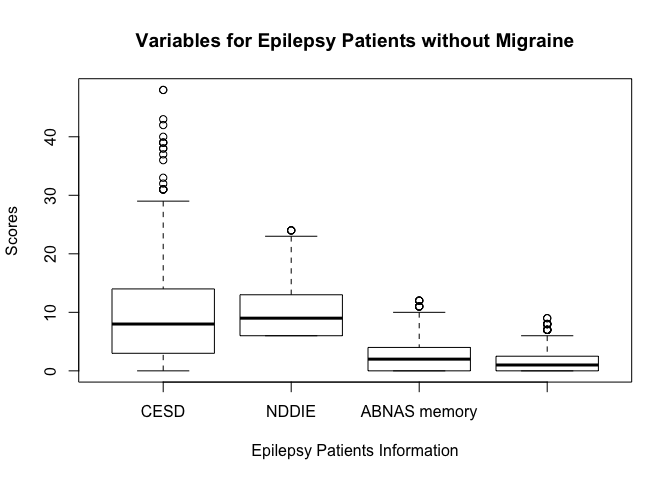
\includegraphics{Methods_hw1_files/figure-latex/unnamed-chunk-17-2.pdf}

Comments:

\begin{enumerate}
\def\labelenumi{\arabic{enumi}.}
\item
  The median of each variable of epilepsy patients with migraine is
  higher than the median of each varibale of epilepsy patients without
  migraine.
\item
  No matter with or without migraine, the score distribution for each
  variable is slightly right skewed.
\item
  The proportion of NDDIE \textgreater{}= 16 or CESD \textgreater{}= 16
  of epilepsy patient with migraine is higher than The proportion of
  NDDIE \textgreater{}= 16 or CESD \textgreater{}= 16 of epilepsy
  patient without migraine.
\item
  There are more outliers of CESD of epilepsy patients without migraine.
\end{enumerate}

Recommendation:

It seems that the statistics of variables of epilepsy patient with
migraine, such as median, mean, \textgreater{}= 16 proportion of CESD
and NDDIE, is higher than the statistics of variables of epilepsy
patient without migraine. The migraine symptom might indicate the
associations between depression and cognitive performance.


\end{document}
